\begin{frame}[c]
\frametitle{Approach}
\begin{tikzpicture}[grn]

 % placement des noeuds
 
  \node[block,align=center] (rstc) at (-2,5) {\begin{tabular}{c}
                                            \textbf{Biological network} \\ \hline
                                            RSTC network
                                           \end{tabular}};
  
  \node[block] (data) at (4,5) {\begin{tabular}{c}
                                            \textbf{Experimental Data} \\ \hline
                                            Time series data(TSD)
                                           \end{tabular}};
  
 \node[instruct,align=center] (phmodel) at (-2,2.5) {\begin{tabular}{c}
                                            \textbf{Hybrid Model} \\ \hline
                                            AN Model
                                           \end{tabular}};
                                           
  \node[instruct] (estimation) at (2.5,2.5) {\begin{tabular}{c}
                                            \textbf{Estimation of parameters}\\ \hline
                                            $r$ and $sa$ 
                                           \end{tabular}};
                                           
   
 % \node[instruct] (discretization) at (6.5,2.5) {\begin{tabular}{c}
  %                                          \textbf{Discretization} \\ \hline
   %                                         TSD
    %                                       \end{tabular}};
                                           
  \node[instruct] (simulation) at (-2,0) {\textbf{Simulation}};
    
  
  \node[test] (test) at (3,0) {Model validation};
  
 %placement des arrêtes
  \draw[suite] (rstc) --node[inner,left]{1} (phmodel);
  \draw[suite] (phmodel) --node[inner,left]{4} (simulation);
  \draw[suite] (simulation) --node[inner,above]{5} (test.west);
  
  \draw[suite] (data) --node[inner,left]{2} (estimation);
  \draw[suite] (estimation) --node[inner,above]{3} (phmodel);
  %\draw[suite] (data) --node[inner,left,node distance=5mm]{2'} (discretization);
  %\draw[suite] (discretization) --node[inner,left,node distance=1cm]{5} (test.east);
\end{tikzpicture}

\end{frame}


\begin{frame}[c]
 \frametitle{RSTC Network}
 \framesubtitle{multi-layer receptor-signaling-transcription-cell state}
%\begin{beamer}

\begin{center}
  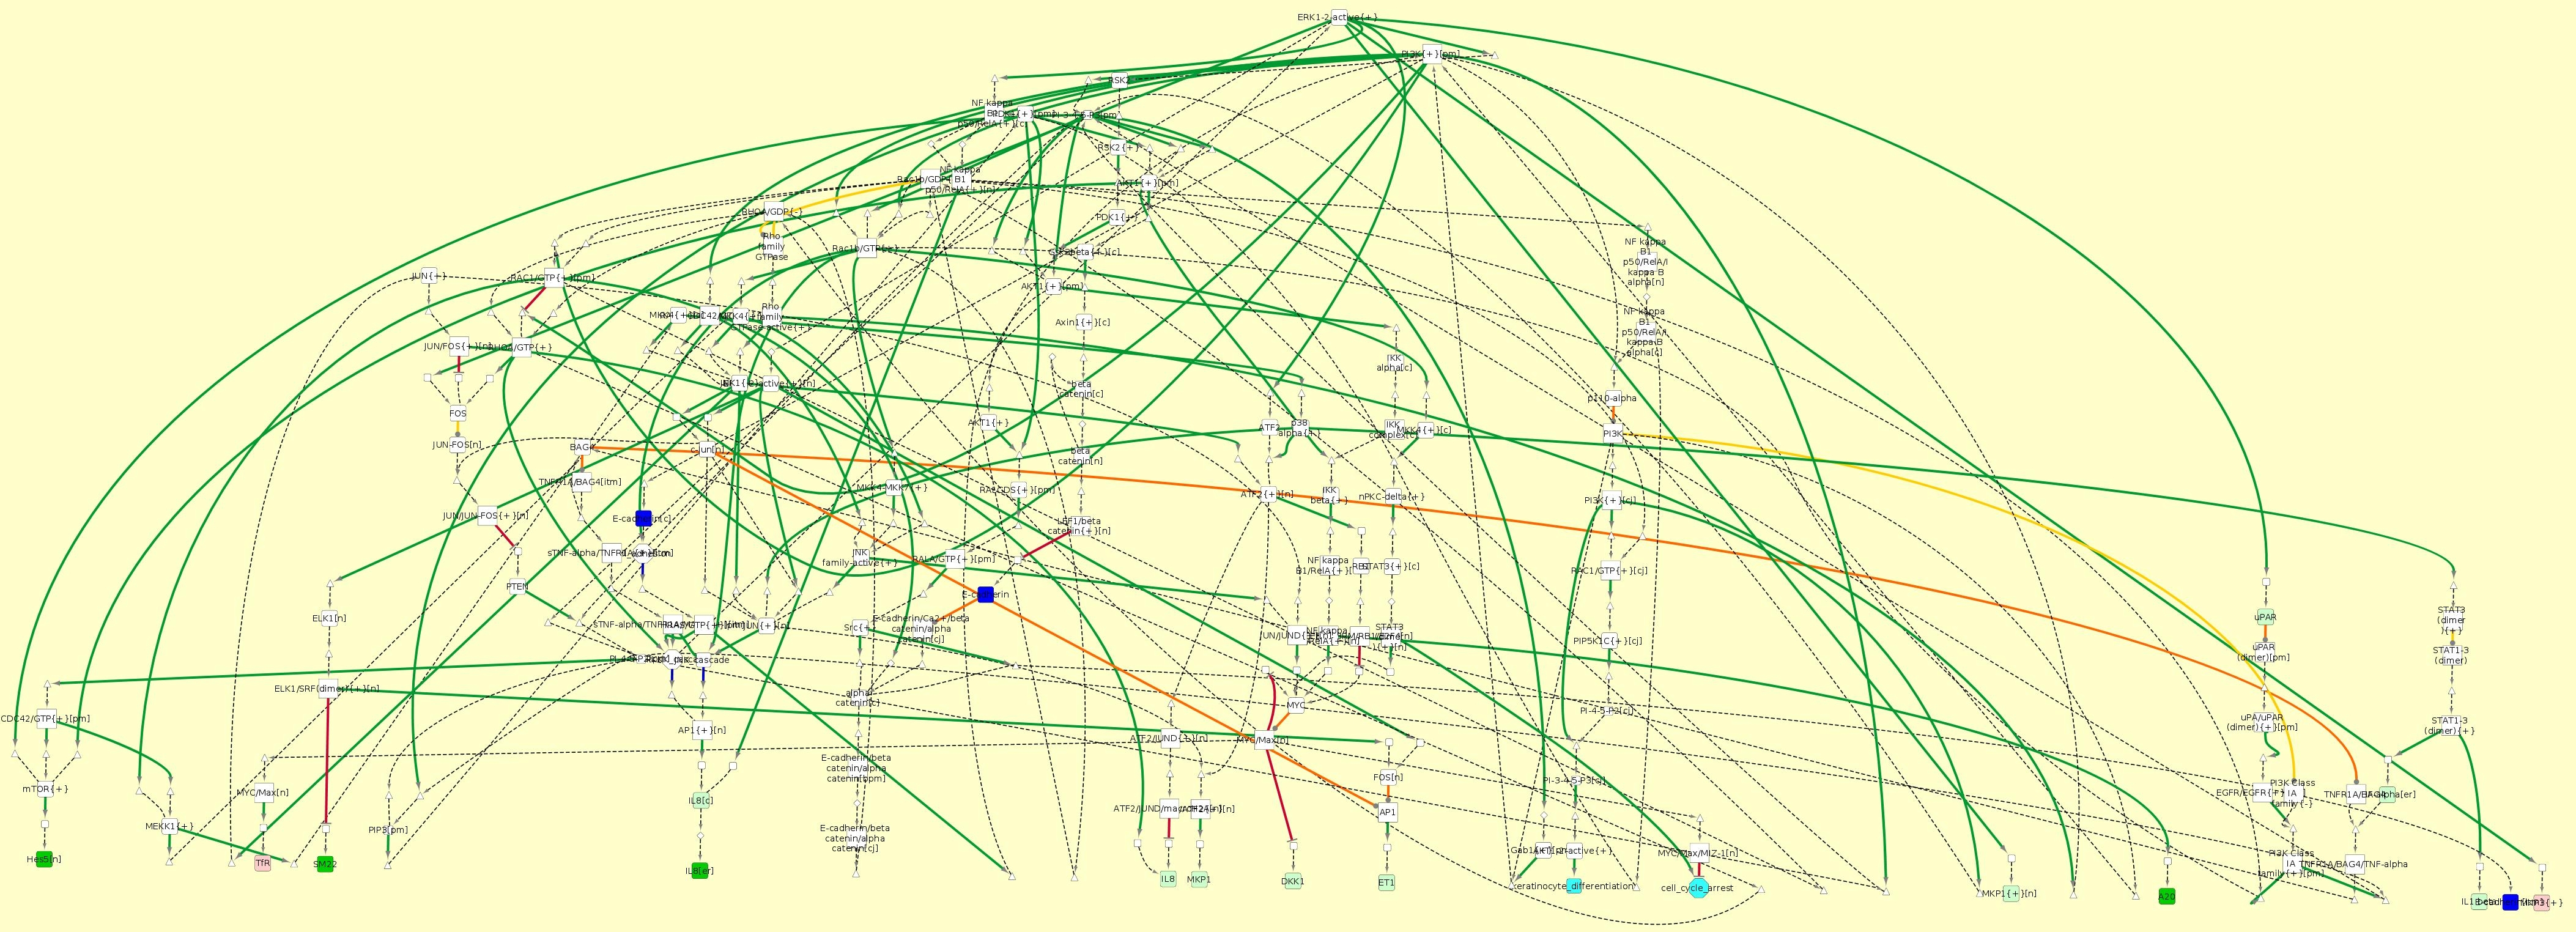
\includegraphics[scale=0.07]{figs/net.jpg}
\end{center}
 
%\end{beamer}

%\pause

\begin{itemize}
 \item Pathway Interaction Database
 \item \tval{$293$  nodes}: signaling proteins, transcription factors, mRNA expressions
 \item \tval{$375$  interactions}: activations, inhibitions, complexes dissociation
\end{itemize}

 
\end{frame}

\begin{frame}[c]
 \frametitle{RSTC Network}
 \framesubtitle{multi-layer receptor-signaling-transcription-cell state}

%%%image zoomée
\begin{tikzpicture}[node distance = 1em,dashed,red,thick]
	\zoomZero{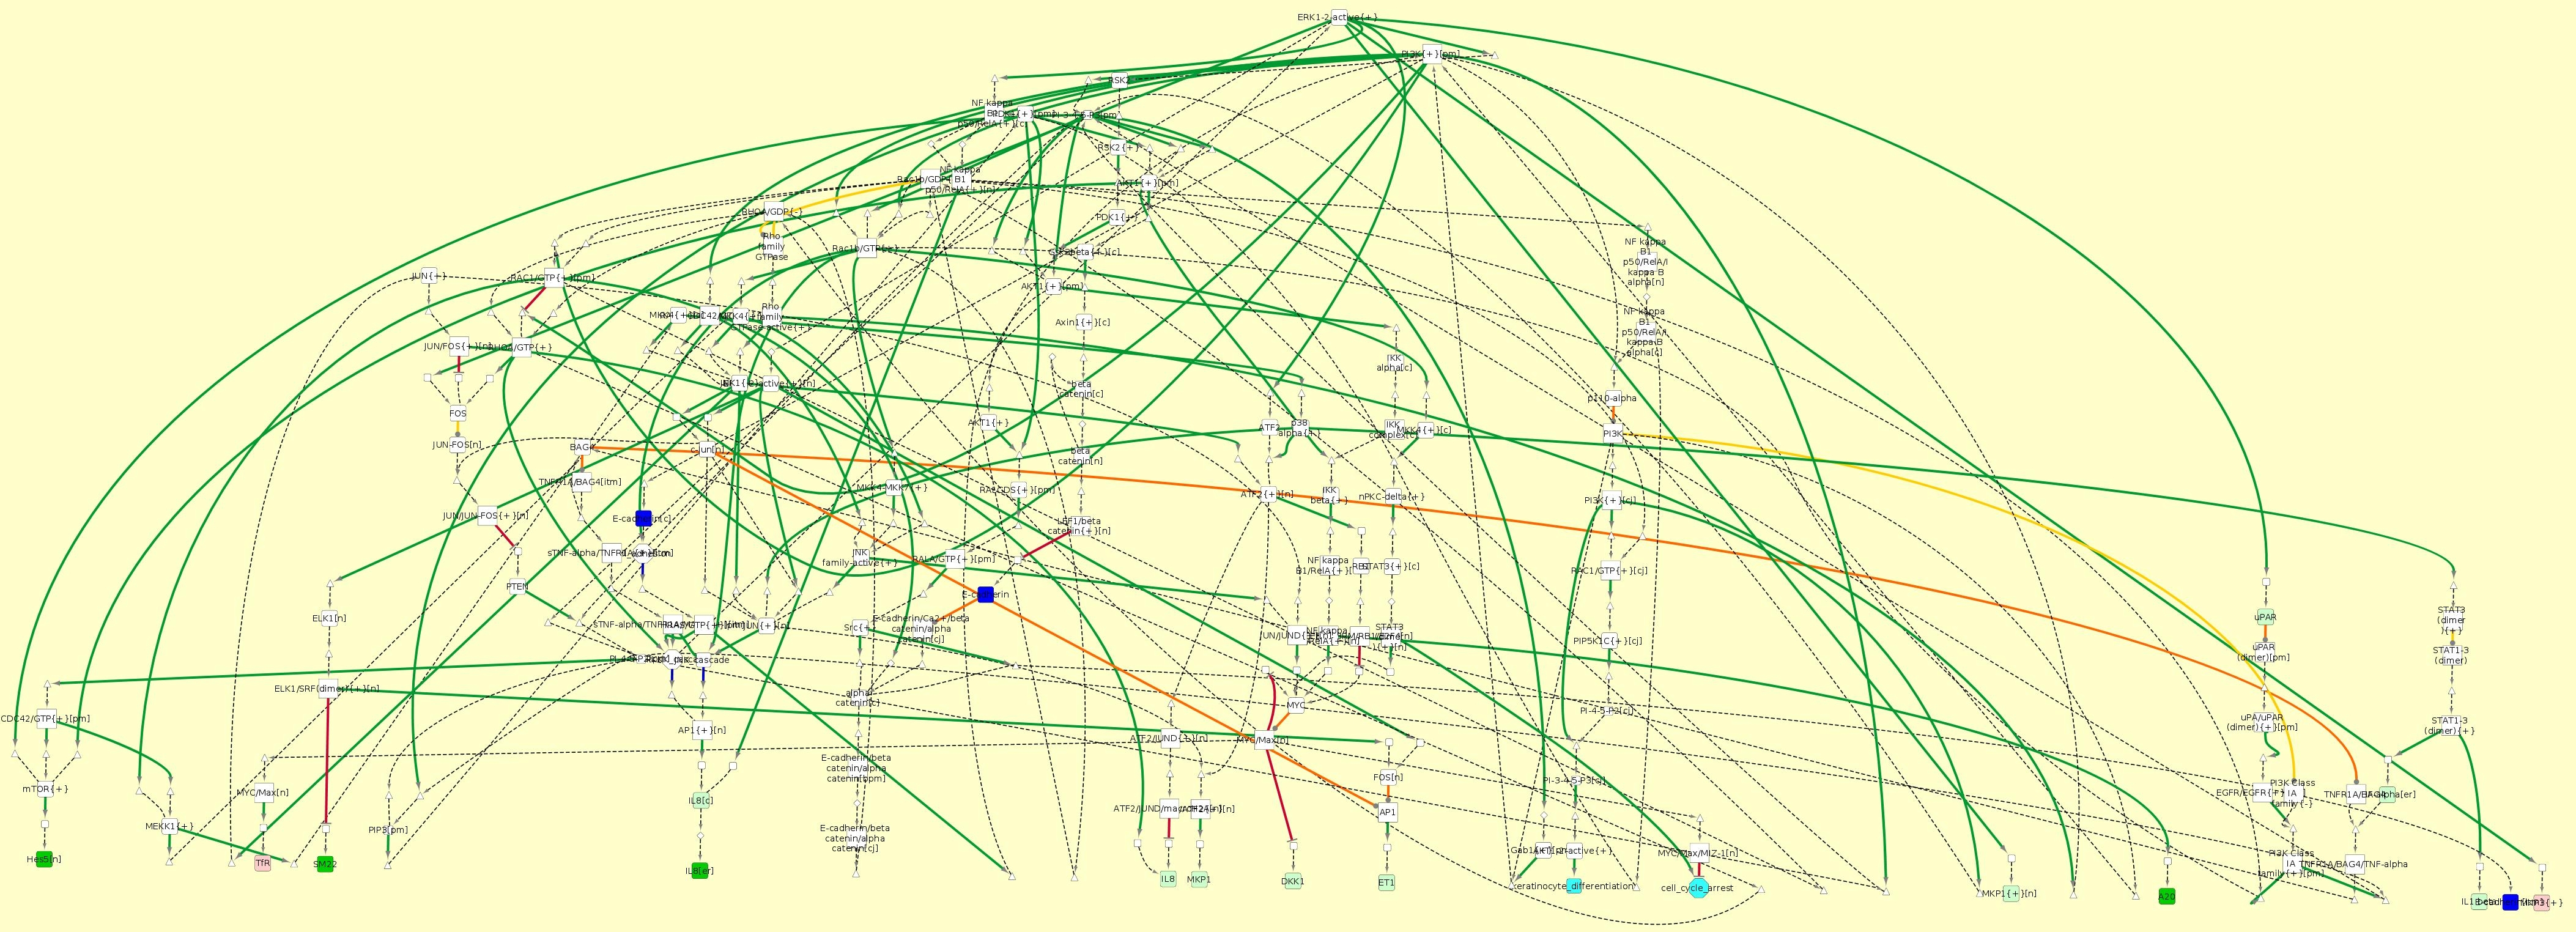
\includegraphics[width=0.35\textwidth]{figs/net.jpg}}
	\zoomIn[right]{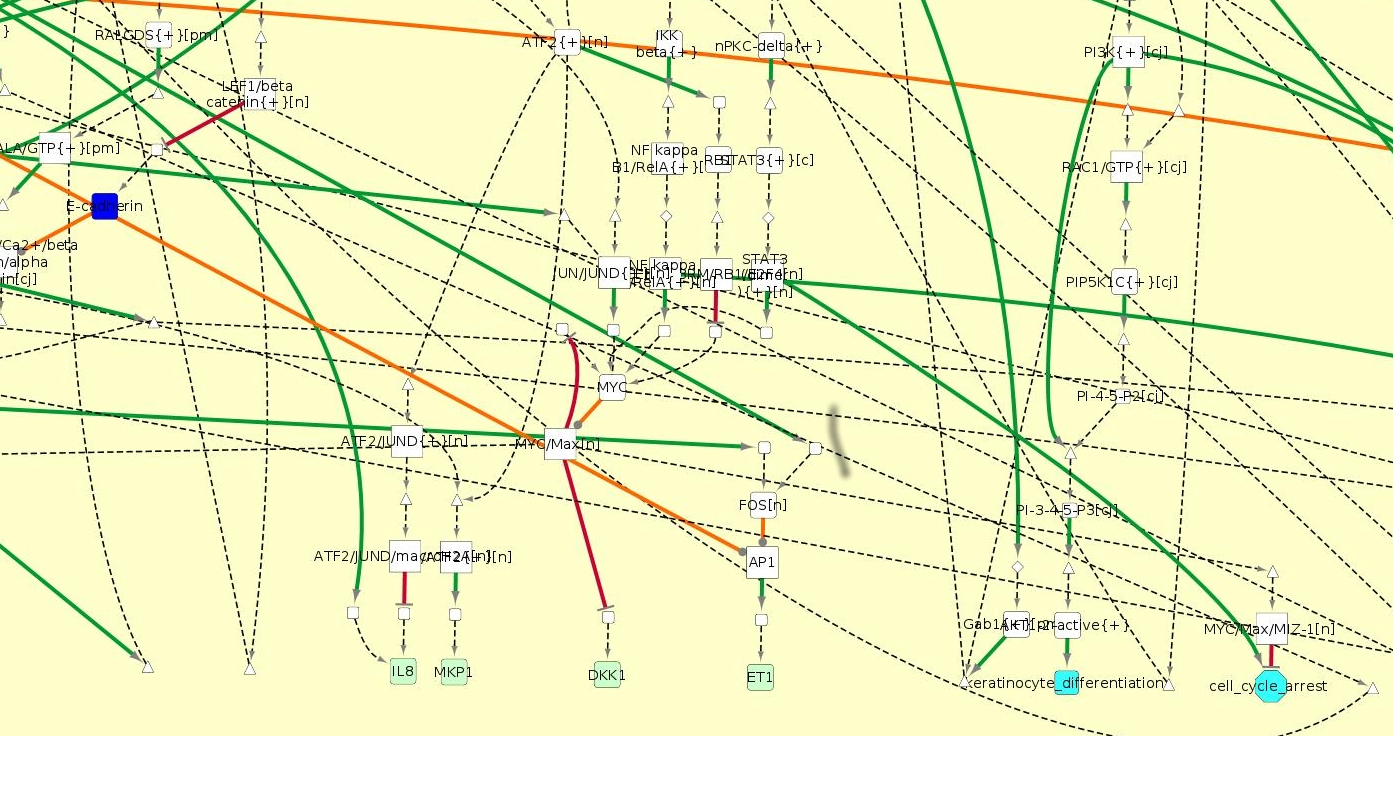
\includegraphics[scale=0.15]{figs/netzoom.png}}{0.35,0.005}{0.320,0.420}
	%\zoomIn{\includegraphics[width=0.45\textwidth]{Geant3}}{0.45,0.475}{0.120,0.120}
	%\zoomIn[left]{\includegraphics[width=0.45\textwidth]{Geant2}}{0.45,0.475}{0.120,0.120}
	%\zoomIn{\includegraphics[width=0.45\textwidth]{Geant1}}{0.45,0.475}{0.120,0.120}
	%\zoomIn[right]{\includegraphics[width=0.45\textwidth]{Geant0}}{0.45,0.475}{0.120,0.120}
\end{tikzpicture}


\end{frame}

\begin{frame}[c]
 \frametitle{RSTC Network}
 \framesubtitle{multi-layer receptor-signaling-transcription-cell state}

%%%image zoomée
\begin{tikzpicture}[node distance = 1em,dashed,red,thick]
	\zoomZero{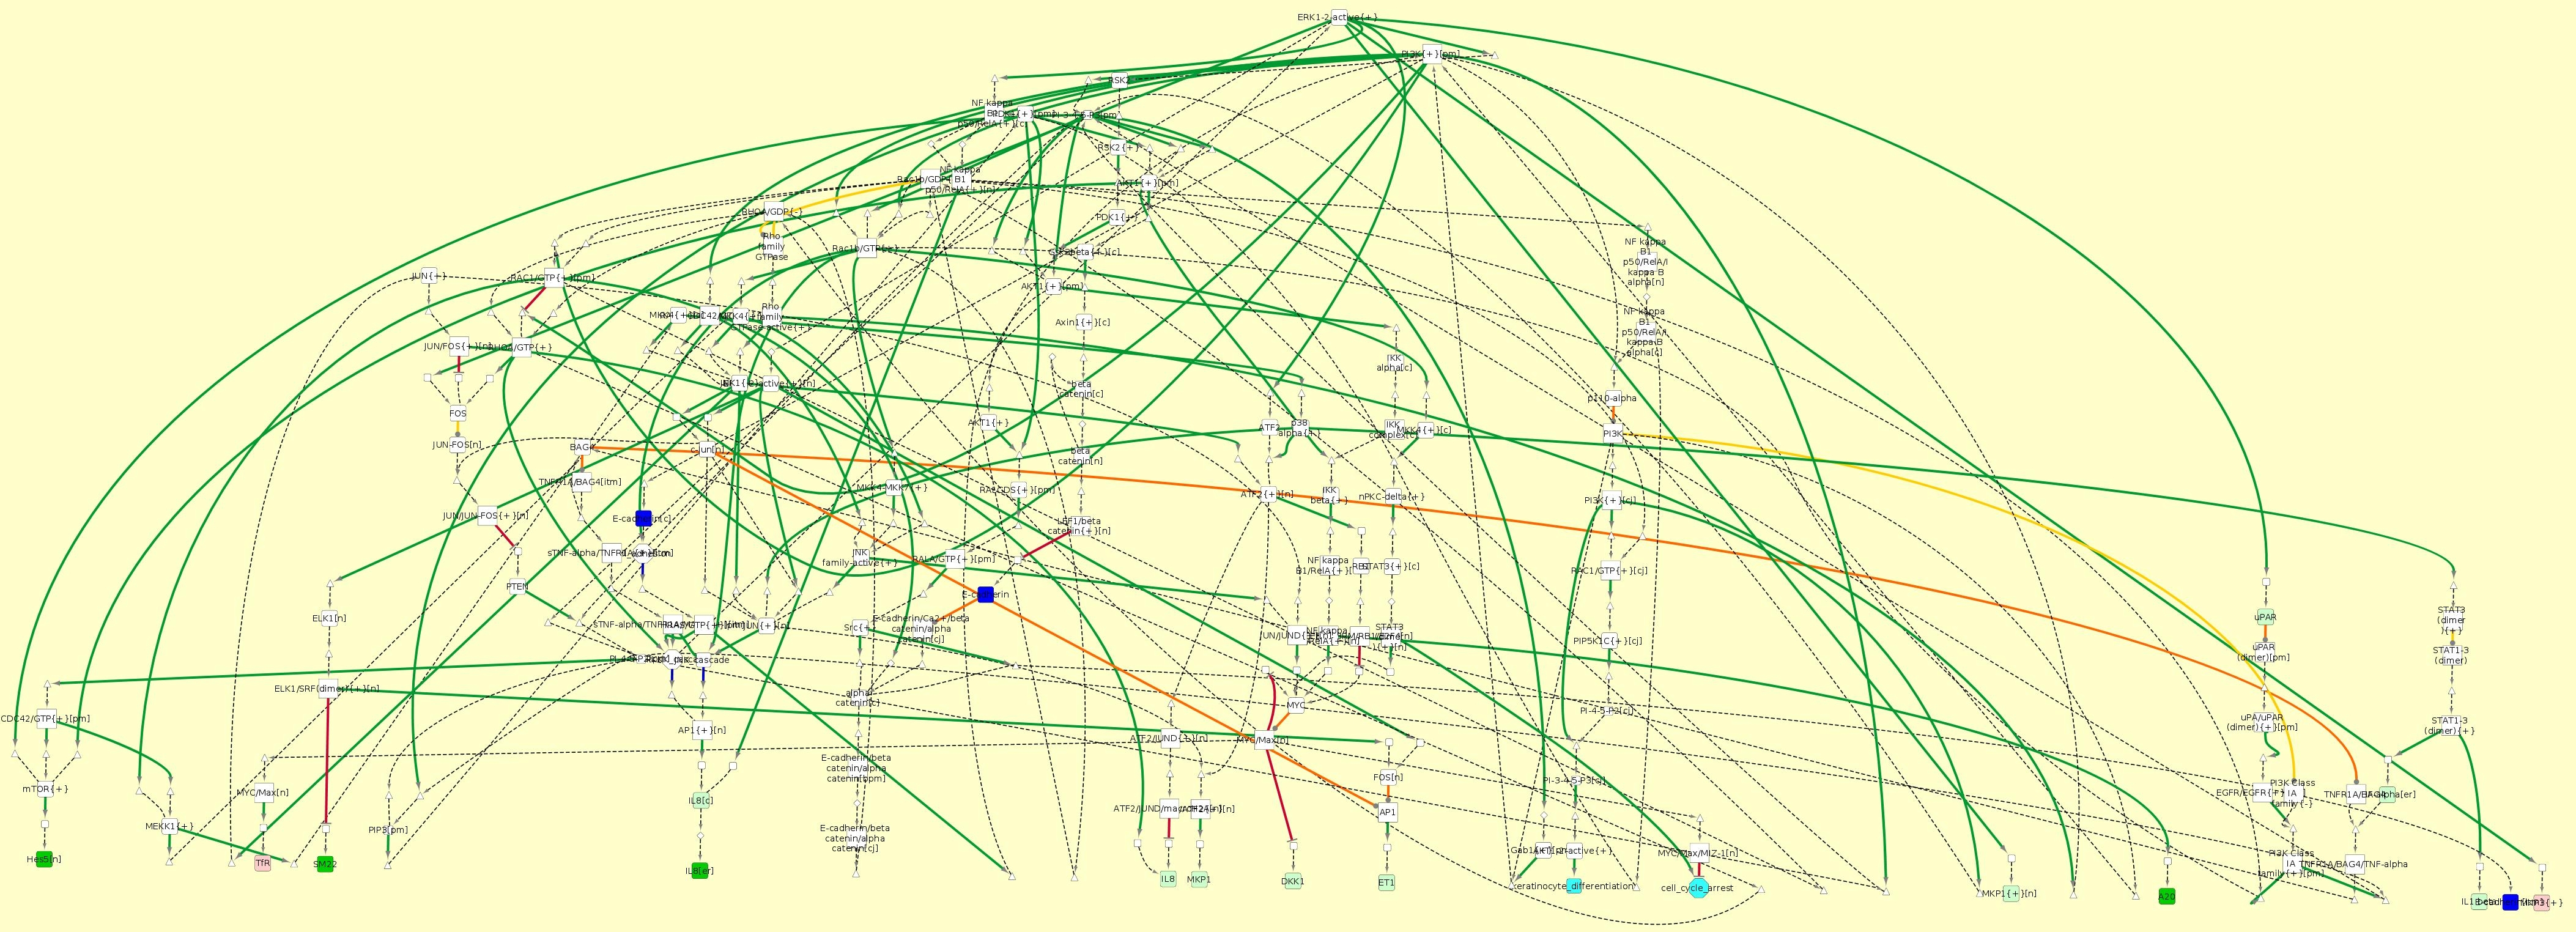
\includegraphics[width=0.45\textwidth]{figs/net.jpg}}
	\zoomIn[left]{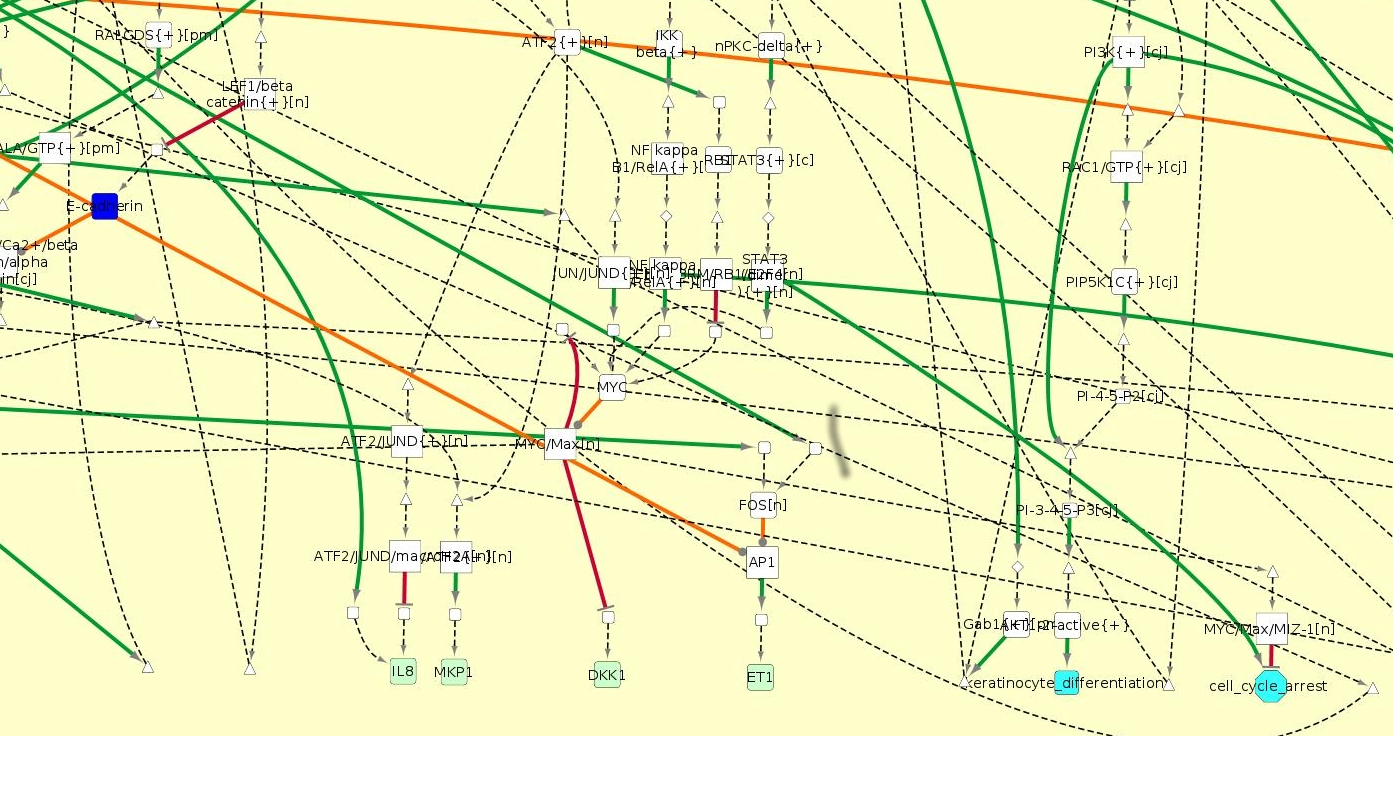
\includegraphics[scale=0.25]{figs/netzoom.png}}{0.35,0.005}{0.320,0.420}
	%\zoomIn{\includegraphics[width=0.45\textwidth]{Geant3}}{0.45,0.475}{0.120,0.120}
	%\zoomIn[left]{\includegraphics[width=0.45\textwidth]{Geant2}}{0.45,0.475}{0.120,0.120}
	%\zoomIn{\includegraphics[width=0.45\textwidth]{Geant1}}{0.45,0.475}{0.120,0.120}
	%\zoomIn[right]{\includegraphics[width=0.45\textwidth]{Geant0}}{0.45,0.475}{0.120,0.120}
\end{tikzpicture}


\end{frame}


\begin{frame}[c]
  \frametitle{Time series data}
  
\begin{center}
  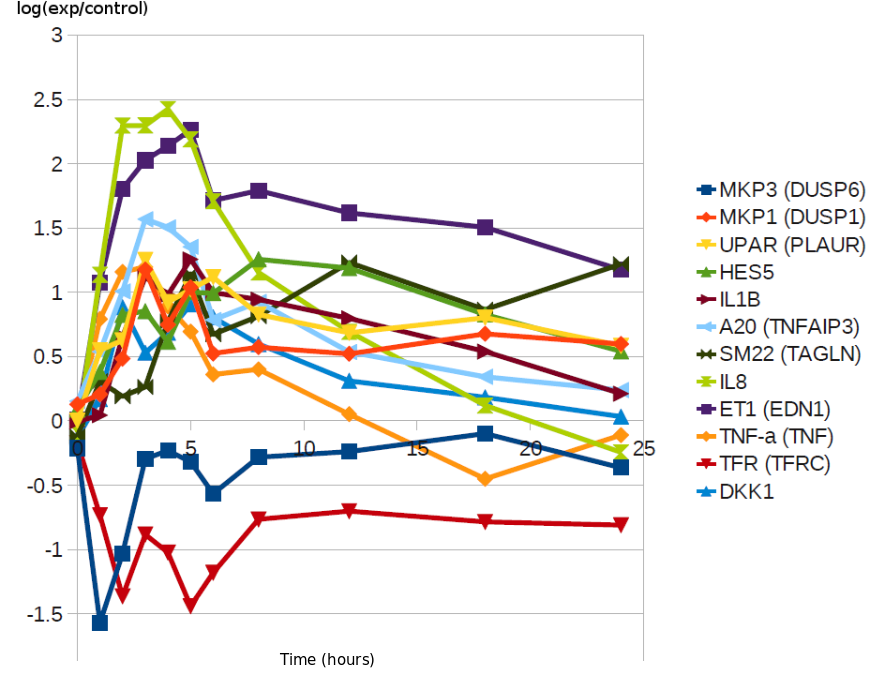
\includegraphics[width=70mm]{figs/12genes.png}
\end{center}

%\pause

\begin{columns}
\begin{column}{0.7\textwidth}
\begin{itemize}
  \item Experiment: \tval{calcium stimuli}
  \item Measured at 10 time-points(0-24hrs)
  \item \tval{$200$ transcripts} selected  (\tval{dynamic patterns}) %their fold expression with respect to the non-stimulated cell was significant in at least one time point
  \item We included in our model a subset of $12$ of them
\end{itemize}
\end{column}

\begin{column}{0.3\textwidth}
% \textbf{ \small Prof. Dr. Peter Angel
%Signal Transduction and Growth Control (A100)
%German Cancer research center
%Heidelberg, Germany}

\end{column}
\end{columns}
%\textcolor{couleurtheme}{$\Rightarrow$} \fbox{\tval{\large Allow efficient translation from Process Hitting to BRN}} \textcolor{couleurtheme}{$\Leftarrow$}

\end{frame}



\begin{frame}[c]
 \frametitle{Data estimation from TSD}
% \framesubtitle{Parameters inference/Principe}
 
\begin{columns}

\begin{column}{0.7\textwidth}
\scalebox{0.9}{
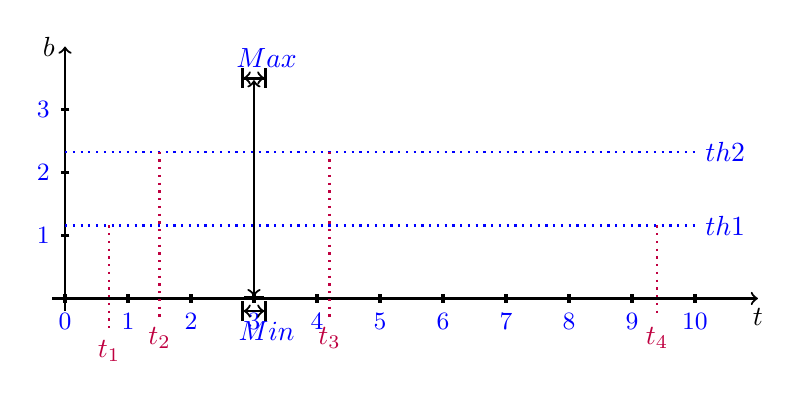
\begin{tikzpicture}[scale = 0.8]
    % Tracé de la parabole
    %\draw[red, domain = -2.2:2.2, smooth] plot (\x, {(\x)^2});
    % Alternative par Gnuplot
    %\draw[red, domain = -2.2:2.2, smooth] plot function{x**2};
    % Lignes tiretées
      \draw[thick, ->] (-.2,0)--(11,0) node[below]{$t$};
     \foreach \t in {0,1,2,3,4,...,10}
      \draw[very thick] (\t,2pt)--(\t,-2pt) node[below,blue]{\small\t};

     \draw[thick, ->] (0,-.2)--(0,4) node[left]{$b$};
     \foreach \y in {1,2,3}
      \draw[very thick] (2pt,\y)--(-2pt,\y) node[left,blue]{\small\y};
      
    \draw[thick] plot[mark=ball,mark size=1pt] file {illustration.txt};
    
    \onslide<2->{
    \draw[thick,|<->|] (2.8,3.5) -- (3.2,3.5) node[above,blue]{$Max$};
    \draw[thick,|<->|] (2.8,-.2) -- (3.2,-.2) node[below,blue]{$Min$};
    }
    \onslide<3->{
    \draw[thick,|<->|] (3,0) -- (3,3.5);
    }
    \onslide<4->{
    \draw[thick,dotted,blue] (0,1.16) -- (10,1.16) node[right]{$th1$}; 
    \draw[thick,dotted,blue] (0,2.33) -- (10,2.33) node[right]{$th2$}; 
    }
    \onslide<5->{
    \draw[thick,dotted,purple] (0.7,1.16) -- (0.7,-.5) node[below]{$t_{1}$};
    }
    \onslide<6->{
    \draw[thick,dotted,purple] (1.5,2.33) -- (1.5,-.3) node[below]{$t_{2}$};
    }
    \onslide<7->{
    \draw[thick,dotted,purple] (4.2,2.33) -- (4.2,-.3) node[below]{$t_{3}$};
    }
    \onslide<8->{
    \draw[thick,dotted,purple] (9.4,1.16) -- (9.4,-.3) node[below]{$t_{4}$};
    }
\end{tikzpicture}
}
%If we assume that $t_{0}=0$,\\
\onslide<5->{$\PHfrappe{a_1}{b_0}{b_1}$ with $r_{1}=\frac{1}{t_{1}-t_{0}}$\\}
\onslide<6->{$\PHfrappe{a_1}{b_1}{b_2}$ with $r_{2}=\frac{1}{t_{2}-t_{1}}$\\}
\onslide<7->{$\PHfrappe{a_0}{b_2}{b_1}$ with $r_{3}=\frac{1}{t_{3}-t_{2}}$\\}
\onslide<8->{$\PHfrappe{a_0}{b_1}{b_0}$ with $r_{4}=\frac{1}{t_{4}-t_{3}}$\\}
\onslide<8->{The formula to estimate the rate of the dynamics of a component according to it TSD is 
\tval{ \Large {$r_{i}=\frac{1}{t_{i}-t_{i-1}}$}}}
\end{column}

\begin{column}{0.3\textwidth}
\scalebox{0.9}{
 \begin{tikzpicture}[scale=0.8]
\path[use as bounding box] (-1,-1) rectangle (2,2);


\TSort{(0,1)}{b}{3}{r}


\only<5->{\TSort{(2,1)}{a}{2}{l}}
\only<5>{
\THit{a_1}{}{b_0}{.east}{b_1}
%\THit{a_0}{out=-120,in=180,selfhit}{a_0}{.west}{a_1}
\path[bounce]
%\TBounce{a_0}{bend left}{a_1}{.south}
\TBounce{b_0}{bend right}{b_1}{.south}
;
\TState{5}{a_1,b_0}
\TState{5}{a_1,b_1}
}

%deuxième estimation
\only<6>{
\THit{a_1}{}{b_1}{.east}{b_2}
%\THit{a_0}{out=-120,in=180,selfhit}{a_0}{.west}{a_1}
\path[bounce]
%\TBounce{a_0}{bend left}{a_1}{.south}
\TBounce{b_1}{bend right}{b_2}{.south}
;
\TState{6}{a_1,b_1}
\TState{6}{a_1,b_2}
}

%troisième  estimation
\only<7>{
\THit{a_0}{}{b_2}{.east}{b_1}
%\THit{a_0}{out=-120,in=180,selfhit}{a_0}{.west}{a_1}
\path[bounce]
%\TBounce{a_0}{bend left}{a_1}{.south}
\TBounce{b_2}{bend right}{b_1}{.north}
;
\TState{7}{a_0,b_2}
\TState{7}{a_0,b_1}
}

%troisième  estimation
\only<8>{
\THit{a_0}{}{b_1}{.east}{b_0}
%\THit{a_0}{out=-120,in=180,selfhit}{a_0}{.west}{a_1}
\path[bounce]
%\TBounce{a_0}{bend left}{a_1}{.south}
\TBounce{b_1}{bend right}{b_0}{.north}
;
\TState{8}{a_0,b_1}
\TState{8}{a_0,b_0}
}

\end{tikzpicture}
}

\end{column}
\end{columns}
\end{frame}







\begin{frame}[c]
  \frametitle{Simulations and analysis}
  
 \begin{center}
  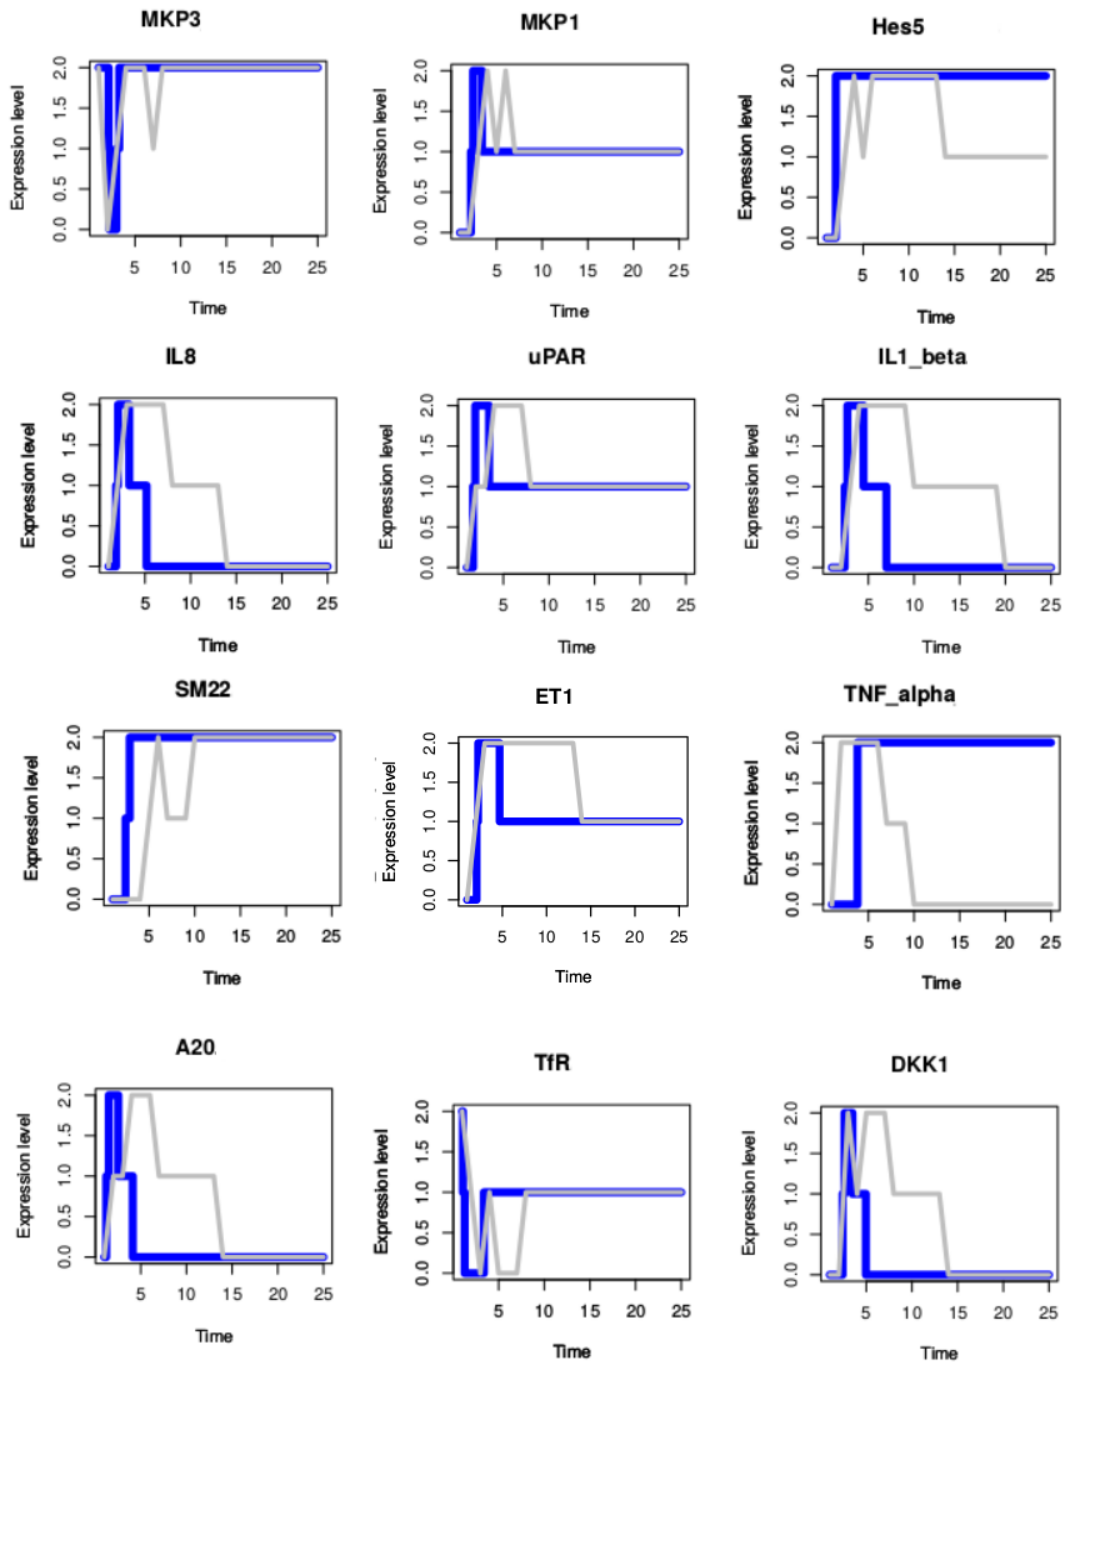
\includegraphics[scale=0.15]{figs/12genes_sim.png}
\end{center}

\textbf{Simulations}

\begin{itemize}
  \item For $r_{a} = r_{i}=10.0$ et $sa = 50 $ for all signalling proteins
  \item With estimated $r$ and $sa$ for MKP3, MKP1, uPAR, Hes5,... according to their expression profiles
  
\end{itemize}

%\textcolor{couleurtheme}{$\Rightarrow$} \fbox{\tval{\large Analyse???}} \textcolor{couleurtheme}{$\Leftarrow$}

\end{frame}




\begin{frame}[c]
  \frametitle{Simulations and analysis}
  
 \begin{center}
  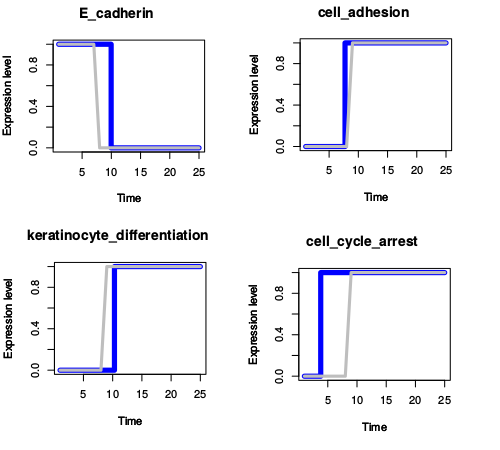
\includegraphics[scale=0.35]{figs/key_nodes1.png}
\end{center}

\textbf{Simulations}

\begin{itemize}
  \item Input node of the system (E\_cadherin)
 \item For biological processes (Cell adhesion, Cell cycle arrest, Keratinocyte differentiation)
  
\end{itemize}

%\textcolor{couleurtheme}{$\Rightarrow$} \fbox{\tval{\large Analyse???}} \textcolor{couleurtheme}{$\Leftarrow$}

\end{frame}


\begin{frame}
   \frametitle{Simulation and Trace analysis}
   %\framesubtitle{work with Guillaume Taupiac}


\begin{columns}
\begin{column}{0.5\textwidth}

\scalebox{0.9}{
\begin{tikzpicture}[scale = 0.8]
       
    \draw[thick, ->] (-.2,-.1)--(7,-.1) node[below]{$t$};
     \foreach \t in {1,2,3,4,5,6}
      \draw[very thick] (\t,-1pt)--(\t,-2pt) node[below,blue]{\small\t};

     \draw[thick, ->] (0,-.2)--(0,3) node[left]{$Level$};
     \foreach \y in {0,1,2}
      \draw[very thick] (2pt,\y)--(-2pt,\y) node[left,blue]{\small\y};
    
    
    \draw[thick,dotted,blue] (0,0) -- (2,0) node[below]{}; 
    \draw[thick,dotted,blue] (2,0) -- (2,1) node[below]{}; 
    \draw[thick,dotted,blue] (2,1) -- (4,1) node[below]{};
    \draw[thick,dotted,blue] (4,1) -- (4,0) node[below]{};
    \draw[thick,dotted,blue] (4,0) -- (6,0) node[below]{};
    \node[instruct,align=center] (mot2) at (4,2) {$\omega=010$};

\end{tikzpicture}
}


%deuxième exemple 
\scalebox{0.9}{
\begin{tikzpicture}[scale = 0.8]
       
    \draw[thick, ->] (-.2,-.1)--(7,-.1) node[below]{$t$};
     \foreach \t in {1,2,3,4,5,6}
      \draw[very thick] (\t,-1pt)--(\t,-2pt) node[below,blue]{\small \t};

     \draw[thick, ->] (0,-.2)--(0,3) node[left]{$Level$};
     \foreach \y in {0,1,2}
      \draw[very thick] (2pt,\y)--(-2pt,\y) node[left,blue]{\small \y};
    
    
    \draw[thick,dotted,blue] (0,0) -- (1,0) node[below]{}; 
    \draw[thick,dotted,blue] (1,0) -- (1,1) node[below]{}; 
    \draw[thick,dotted,blue] (1,1) -- (2,1) node[below]{};
    \draw[thick,dotted,blue] (2,1) -- (2,2) node[below]{};
    \draw[thick,dotted,blue] (2,2) -- (3,2) node[below]{};
    \draw[thick,dotted,blue] (3,2) -- (3,1) node[below]{};
    \draw[thick,dotted,blue] (3,1) -- (5,1) node[below]{};
    \draw[thick,dotted,blue] (5,1) -- (5,0) node[below]{};
    \draw[thick,dotted,blue] (5,0) -- (6,0) node[below]{};
    \node[instruct,align=center] (mot2) at (5,2) {$\omega=01210$};
   

\end{tikzpicture}
}


\end{column}


\begin{column}{0.5\textwidth}

for each component \tval{$C_{i}$, $1 \leq i \leq P$},
\tval{$N$} simulations will generate \tval{$\omega_{i1}, \omega_{i2}, \ldots ,\omega_{iN}$} words.




for $1 \leq j \leq N$

%\newline
%\vspace{1cm}



\scalebox{0.9}{
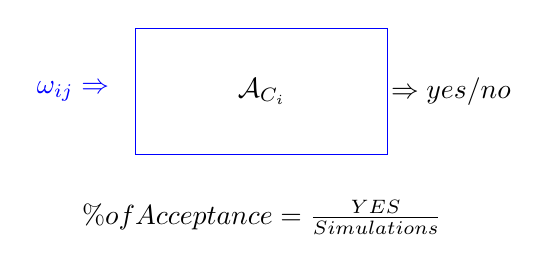
\begin{tikzpicture}[scale = 0.8]
    
    \node[align=center,blue] (mot) at (2,3) {$\omega_{ij} \Rightarrow $};
    
    \draw[blue] (3,2) rectangle (7,4);

    \node[align=center] (automaton) at (5,3) {$\mathcal{A}_{C_{i}}$};
    
    \node[align=center] (accept) at (8,3) {$\Rightarrow \tval{yes}/\alert{no} $};
    
    \node[align=center] (percent) at (5,1) {\tval{$\% of Acceptance = \frac{\card{YES}}{\card{Simulations}}$}};
   

\end{tikzpicture}
}



\end{column}
\end{columns}
\end{frame}

\begin{frame}
\frametitle{Simulation and Trace analysis}
\begin{tabular}{|c|c||c|c|}
\hline

\textbf{Automate} & \textbf{components} & \textbf{$\%$  validation} & \textbf{$\%$ of acceptance $T_{1}$}
\\ \hline

$\mathcal{A}_{2}(01210)$ & A20 & 91 & 100 
\\ \hline

$\mathcal{A}_{2}(01210)$ & IL1$\_$beta & 81 & 100
\\ \hline

$\mathcal{A}_{2}(01210)$ & IL8 & 93 & 100 
\\ \hline

$\mathcal{A}_{2}(01210)$ & TNF$\_$alpha & 0 & 0
\\ \hline

$\mathcal{A}_{3}(01211)$ & uPar & 76 & 99 
\\ \hline

$\mathcal{A}_{3}(01211)$ & ET1 & 8 & 19 
\\ \hline

$\mathcal{A}_{4}(0121210)$ & DKK1 & 13 & 43

\\ \hline

$\mathcal{A}_{5}(0121211)$ & Hes5 & 0 & 17 
\\ \hline

$\mathcal{A}_{5}(0121211)$ & MKP1 & 9 & 97
\\ \hline

$\mathcal{A}_{6}(0212)$ & SM22 & 11 & 100 
\\ \hline

$\mathcal{A}_{7}(02010)$ & MKP3 & 11 & 98

\\ \hline

$\mathcal{A}_{8}(02121)$ & Tfr & 0 & 94 
\\ \hline

\end{tabular}

\end{frame}


